\textbf{\underline{\large{1.8: Related Rates}}} \par

In this course, derivatives have primarily been interpreted as the slope of the tangent line. But, as with \href{https://www.merriam-webster.com/dictionary/rectilinear\%20motion}{\text{\textcolor{blue}{rectilinear motion}}}, there are other contexts for the derivative. One overarching concept is that the derivative is a \textbf{rate of change}. The tendency is to think of rates as distance per time unit, like miles per hour or meters per second, but even slope is a rate of change---it is just that the rise and run are both measured as distances. \par

The idea behind related rates is two-fold. First, change is occurring in two or more measurements that are related to each other by the geometry (or algebra) of the situation. Second, an implicit Chain Rule situation exists in that the $x$ and $y$-values are functions of time, which may or may not be a variable in the problem. Therefore, when taking the derivative of an $x$ or $y$, an \textbf{implicit rate term} $\left(\dfrac{dx}{dx} \text{ or } \dfrac{dy}{dt}\right) \forcespace$ often occurs. \par

\begin{tcolorbox}[objective]
    \begin{center}
        OBJECTIVES \\[11pt]
    \end{center}
    Solve Related Rates Problems.
\end{tcolorbox}

At first glance, related rates problems might seem like optimization problems that we've seen last year. Consider the following example:

\begin{tcolorbox}[example]
    \textbf{Ex 1.8.1: } The volume of a cylindrical cola can is $32\pi \si{in^3}$. What is the minimum surface area for such a can?
\end{tcolorbox}

The word ``minimum'' tells us that we have an optimization problem. Recall our workflow for tackling optimization problems:

\begin{center}
    \begin{tcolorbox}[default]
        \begin{center}
            \textbf{Strategy For Optimization Problems} \\[22pt]
        \end{center}
        \begin{tikzpicture}[node distance=2cm]
        
            \node (read) [startstop] 
                {Read the problem to decide on a primary equation (the one to maximize)};
            \node (decision) [decision, below of=read, yshift=-1cm, xshift=-3.5cm] 
                {Are there more than two variables?};
            \node (secondary) [process, right of=decision, xshift=6cm] 
                {Create a secondary equation};
            \node (picture) [process, below of=secondary] 
                {Draw and label a picture. \\ Do not use $x$ or $y$!};
            \node (isolate) [process, below of=picture] 
                {Isolate the variable to eliminate from the primary equation.};
            \node (substitute) [process, below of=isolate] 
                {Substitute into the primary equation.};
            \node (derivative) [process, below of=decision, yshift=-4cm] 
                {Take the derivative and set it equal to zero.};
            \node (critical) [process, below of=derivative] 
                {Solve for the critical values. \\ \textbf{Don't forget endpoints!}};
            \node (sign) [process, below of=critical] 
                {Check the sign pattern to determine max vs. minimum.};
            \node (answer) [startstop, below of=sign, xshift=3.5cm] 
                {Reread the problem and \textbf{answer the question that was asked.}};

            % Arrows
            \draw [arrow] ([xshift=-3.5cm]read.south) -- (decision.north);
            \draw [arrow] (decision) -- (secondary) node[midway, above] {\textbf{Yes}};
            \draw [arrow] (secondary) -- (picture);
            \draw [arrow] (picture) -- (isolate);
            \draw [arrow] (isolate) -- (substitute);
            \draw [arrow] (substitute) -- (derivative);
            \draw [arrow] (decision.south) -- (derivative) node[midway, left] {\textbf{No}};
            \draw [arrow] (derivative) -- (critical);
            \draw [arrow] (critical) -- (sign);
            \draw [arrow] (sign.south) -- ([xshift=-3.5cm]answer.north);
    
        \end{tikzpicture}
    \end{tcolorbox}
\end{center}

So, let's tackle our example. \par

\begin{tcolorbox}[solution]
    \textbf{Sol 1.8.1: } The problem asks to minimize surface area, which is determined by: \begin{align*}
        S = 2\pi r^2 + 2\pi rh 
    \end{align*}
    As there are more than two variables in this equation, either $r$ or $h$ needs to be eliminated in this formula before differentiating. The volume is $V = \pi r^2h = 32\pi$, so $h = \dfrac{32}{r^2}$ and \begin{align*}
        & S \begin{aligned}[t]
            & = 2\pi r^2 + 2\pi r\left(\dfrac{32}{r^2}\right) \\[11pt]
            & = 2\pi r^2 + \dfrac{64\pi}{r}
        \end{aligned} \\[11pt]
        & S' = 4\pi r - \dfrac{64\pi}{r^2} = 0 \\[11pt]
        & \therefore 4\pi r = \dfrac{64\pi}{r^2} \\[11pt]
        & r^3 = 16 \rightarrow r = 2.5198
    \end{align*}
    Now, let's make a sign pattern to determine if this critical value is a minimum. \\
    \begin{center}
        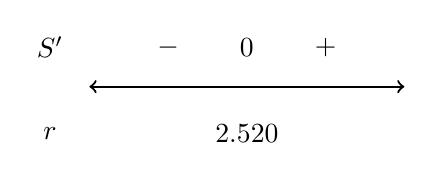
\begin{tikzpicture}[baseline=(current bounding box.center)]
            \draw[<->, thick] (0,0) -- (4,0);

            \node at (2,-0.6) {2.520};
            \node at (-0.5, -0.6) {$r$};

            \node at (1,0.5) {$-$};
            \node at (2,0.5) {$0$};
            \node at (3,0.5) {$+$};
            \node at (-0.5, 0.5) {$S'$};
        \end{tikzpicture}
    \end{center} \vspace{11pt}
    Because the derivative changes from negative to positive, we know that 2.5198 is a minimum. We can plug it back into our surface area equation to find our minimum surface area. \begin{align*}
        & S(2.5198) = 2\pi(2.5198)^2 + \dfrac{64\pi}{2.5198} \\[11pt]
        & S(2.5198) = 119.687 \si{in^2}
    \end{align*}
    Therefore, the minimum surface area of the cola can is $\boxed{119.687 \si{in^2}}$.
\end{tcolorbox}

A related rates problem is characterized by various measurements that are changing \textbf{in relation to each other}. The variables are still related to each other through a geometric or physical relationship. The key difference from other differentiation problems is that we differentiate implicitly with respect to time, rather than a variable like $x$. In other words, 

\begin{center}  
    \fbox{\fbox{\begin{minipage}{0.96 \textwidth}
        \begin{align*}
            & \text{Optimization Problems:} && \text{Apply } \diff \\[11pt]
            & \text{Related Rates Problems:} && \text{Apply } \dfrac{d}{dt} \\
        \end{align*}
    \end{minipage}}}
\end{center}

Now, let's take a look at this different (related rates) cola problem.

\begin{tcolorbox}[example]
    \textbf{Ex 1.8.2: } The volume of a cylindrical cola can is $32\pi \si{in^3}$. The height of the can is changing at $\dfrac{1}{4} \si{in \per sec} \forcespace$. If the radius changes at the same time so as to maintain the volume, how fast is the radius shrinking when the can is $4$ inches tall? 
\end{tcolorbox} 
\begin{tcolorbox}[solution]
    \textbf{Sol 1.8.2: } \begin{align*}
        & V = \pi r^2h = 32\pi \\[11pt]
        & h = \dfrac{32}{r^2} \\[11pt]
        & \tdiff\left[h = \dfrac{32}{r^2}\right] \\[11pt]
        & \dfrac{dh}{dt} = -\dfrac{64}{r^2}\left(\dfrac{dr}{dt}\right)
    \end{align*}
    Now that we have a method to find what we are looking for, $\dfrac{dr}{dt}$, let's substitute in the values that we are given in the problem. \begin{align*}
        & h = 4 \rightarrow \dfrac{32}{r^2} = 4 \rightarrow r^2 = 8 \\[11pt]
        & \dfrac{1}{4} = -\dfrac{64}{8}\left(\dfrac{dr}{dt}\right) \\[11pt]
        & \dfrac{dr}{dt} = \boxed{-\dfrac{1}{32} \si{in \per sec}}
    \end{align*}
\end{tcolorbox}

As we can see, many of the steps that we take in the related rates cola problem is similar to those of the optimization cola problem. 

\textbf{Process For Related Rates Problems} \par

\begin{enumerate}[label=\arabic*.]
    \item Draw a visual for the problem. 
    \item Label the visual with what is given and what is being asked. 
    \begin{enumerate}[label=\alph*.]
        \item Use variables for any quantities that are \textbf{changing}. 
        \item Pay particular attention to the units.
    \end{enumerate}
    \item Determine the equation(s) that relate the variables to each other.
    \begin{enumerate}[label=\alph*.]
        \item Decide which equation will be differentiated.
        \item If there is a product of two variables, eliminate the product by either multiplying the equation out or substituting a secondary equation.
    \end{enumerate}
    \item \textbf{Differentiate in terms of time!} This is the key step.
    \begin{enumerate}[label=\alph*.]
        \item Do not forget implicit fractions.
    \end{enumerate}
    \item Substitute the given information and solve for the missing variable.
    \item Reread the problem and make sure to answer the question that was asked.
\end{enumerate} \vspace{11pt}

A classic related rates problem is the falling ladder. 

\begin{tcolorbox}[example]
    \textbf{Ex 1.8.3: } A $13$-foot ladder is leaning against a wall. The bottom of the ladder slides away from the wall at $4 \si{ft \per sec}$. How fast is the top of the ladder moving down the wall when the ladder is $5$ feet from the wall? \\[11pt]

    \begin{center}
        \begin{tikzpicture}[tdplot_main_coords, scale=1.25]

            % Wall (x-z plane at y=0)
            \fill[gray!5, opacity=0.8] (0,0,0) -- (0,4.5,0) -- (-4.5,4.5,0) -- (-4.5,0,0) -- cycle;

            % Floor (x-y plane at z=0)
            \fill[gray!10, opacity=0.7] (0,0,0) -- (-4.5,0,0) -- (-4.5,0,4.5) -- (0,0,4.5) -- cycle;

            % Axes
            \draw[->] (0,0,0) -- (-5,0,0) node[anchor=south]{$z$};
            \draw[->] (0,0,0) -- (0,0,5) node[anchor=south]{$y$ (ladder height)};
            \draw[->] (0,0,0) -- (0,5,0) node[anchor=west]{$x$ (ladder base)};

            % Ladder
            \draw[very thick, red] (0,0,4) -- (0,1.667,0);
            \draw[very thick, red] (-0.5,0,4) -- (-0.5,1.667,0) node[pos=0.35, above right, sloped] {Ladder};
            \foreach \i in {1,...,7} {
                \draw[very thick, red] ({0}, {0.208*\i}, {4 - 0.5*\i}) -- ({-0.5}, {0.208*\i}, {4 - 0.5*\i});
            }

            % Labels
            \node at (0,2.3,1.5) [red] {$\ell = 13$};
        
        \end{tikzpicture}
    \end{center}           
\end{tcolorbox}
\begin{tcolorbox}[solution]
    \textbf{Sol 1.8.3: } As can be seen in the visual, the height of the top of the ladder and the distance the bottom of the ladder is from the wall is related through the Pythagorean theorem. Both are variables, because the ladder is moving. \begin{align*}
        x^2 + y^2 = 13^2
    \end{align*}
    We are given the information that the bottom of the ladder slides away from the wall at $4 \si{ft \per sec}$. Therefore, we can say that our $\dfrac{dx}{dt} \forcespace = 4$. To find $\dfrac{dy}{dt}$, we differentiate $x^2 + y^2 = 13^2$ to get \begin{align*}
        2x\dfrac{dx}{dt} + 2y\dfrac{dy}{dt} = 0
    \end{align*}
    Although this may seem like a complex four equation variable, we already know $x$ and $\dfrac{dx}{dt} \forcespace$. We also can determine that $y = 12$ by the Pythagorean theorem. So, \begin{align*}
        & 2x\dfrac{dx}{dt} + 2y\dfrac{dy}{dt} = 0 \\[11pt]
        & 2(5)(4) + 2(12)\dfrac{dy}{dt} = 0 \\[11pt]
        & \dfrac{dy}{dt} = \boxed{-\dfrac{5}{3} \si{ft \per sec}}
    \end{align*}
    It should make sense that $\dfrac{dy}{dt}$ is negative because the top of the ladder is sliding down.
\end{tcolorbox}

Below are some of the equations you should know for the AP exam: \par

\begin{center}  
    \fbox{\fbox{\begin{minipage}{0.96 \textwidth}
        \vspace{11pt}
        \begin{center}
            \textbf{Common Formulas For Optimization/Related Rates Problems} \\[11pt]
            \textbf{Pythagorean Theorem} \begin{align*}
                x^2 + y^2 = r^2
            \end{align*} 
            \textbf{Area Formulas} \begin{align*}
                & \text{Circle: } A = \pi r^2 && \text{Rectangle: } A = lw \\[11pt]
                & \text{Triangle: } A = \dfrac{1}{2}bh && \text{Trapezoid: } A = \dfrac{1}{2}h\left(b_1 + b_2\right)
            \end{align*}
            \textbf{Volume Formulas} \begin{align*}
                & \text{Sphere: } V = \dfrac{4}{3}\pi && \text{Right Prism: } V = Bh &&& \text{Cylinder: } V = \pi r^2h \\[11pt]
                & \text{Cone: } V = \dfrac{1}{3}\pi r^2h && \text{Right Pyramid: } V = \dfrac{1}{3}Bh &&& \text{*Washer: } V = \pi(R^2 - r^2)h
            \end{align*}
            \textbf{Surface Area Formulas} \begin{align*}
                & \text{Sphere: } S = 4\pi r^2 && \text{Cylinder: } S = 2\pi r^2 + 2\pi rh \\[11pt]
                & \text{Cone: } S = \pi r^2 + \pi rl && \text{*Right Prism: } S = 2B + Ph \\[11pt]
            \end{align*}
            \footnotesize{N.B. The two equations with asterisks are less commonly used.}
        \end{center} 
        \vspace{11pt}
    \end{minipage}}}
\end{center}

Another common related rates problem is where a tank of a particular shape is filling or draining. \par

\begin{tcolorbox}[example]
    \textbf{Ex 1.8.4: } A tank shaped like an inverted cone $8$ feet in height and with a base diameter of $8$ feet is filling at a rate of $10 \si{ft^3 \per min}$. How fast is the height changing when the water is $6$ feet deep? \\[11pt]

    \begin{center}
        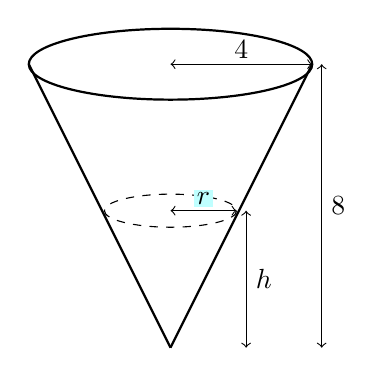
\begin{tikzpicture}[scale=0.6]
            \draw[thick] (-3,0) arc[start angle=180,end angle=540,x radius=3cm,y radius=0.75cm];

            \draw[thick] (-3,0) -- (0,-6);
            \draw[thick] (3,0) -- (0,-6);
            \draw[dashed] (-1.4,-3.1) arc[start angle=180,end angle=540,x radius=1.4cm,y radius=0.35cm];

            \draw[<->] (0, -3.1) -- (1.4, -3.1) node[midway, above, yshift=1pt, fill=Cyan!25, inner sep=1pt] {$r$};
            \draw[<->] (1.6, -3.1) -- (1.6, -6) node[midway, right] {$h$};
            \draw[<->] (0, 0) -- (3, 0) node[midway, above, yshift=-1.5pt] {$4$};
            \draw[<->] (3.2, 0) -- (3.2, -6) node[midway, right] {$8$};

        \end{tikzpicture}
    \end{center}

\end{tcolorbox}
\begin{tcolorbox}[solution]
    \textbf{Sol 1.8.4: } The units on the rate of change tell us that this is a change in volume, or $\dfrac{dV}{dt}$. Therefore, we use the equation \begin{align*}
        V = \dfrac{1}{3}\pi r^2h
    \end{align*}
    But, there are too many variables in this equation to differentiate as it stands. Since the rate of the change of the height---$\dfrac{dh}{dt} \forcespace$---is what we are looking for, we can eliminate $r$ from the equation. By similar triangles, we have \begin{align*}
        & \dfrac{r}{h} = \dfrac{4}{8} \\[11pt]
        & r = \dfrac{1}{2}h
    \end{align*}
    Substitution gives us a volume equation in terms of only height. \begin{align*}
        & V = \dfrac{1}{3}\pi\left(\dfrac{1}{2}h\right)^2h \\[11pt]
        & V = \dfrac{\pi}{12}h^3
    \end{align*}
    Differentiate and plug in our given values to solve for $\dfrac{dh}{dt}$. \begin{align*}
        & V = \dfrac{\pi}{12}h^3 \\[11pt]
        & \dfrac{dV}{dt} = \dfrac{\pi}{4}h^2\dfrac{dh}{dt} \\[11pt]
        & 10 = \dfrac{\pi}{4}(6)^2\dfrac{dh}{dt} \\[11pt]
        & \dfrac{dh}{dt} = \boxed{\dfrac{10}{9\pi} \si{ft \per min}}
    \end{align*}
\end{tcolorbox} \vspace{11pt}

\begin{tcolorbox}[example]
    \textbf{Ex 1.8.5: } Two cars approach an intersection, one traveling south at $20$ miles per hour and the other traveling west at $30$ miles per hour. How fast is the direct distance between them decreasing when the westbound car is $0.6$ miles and the southbound car is $0.8$ miles away from the intersection? \\[11pt]

    \begin{center}
        \begin{tikzpicture}[scale=0.5]
            
            \draw[arrow] (0, 0) -- (0, -8) node[midway, left, xshift=-11pt] {$y$};
            \draw[arrow] (6, -8) -- (0, -8) node[midway, below] {$x$};
            \draw[dashed] (0, 0) -- (6, -8) node[midway, above] {$r$};

            \fill[WildStrawberry!80] (-0.38, 0.38) -- (0.38, 0.38) -- (0.38, -0.75) -- (-0.38, -0.75) -- cycle;
            \fill[Blue!60] (5.25, -7.68) -- (6.38, -7.68) -- (6.38, -8.38) -- (5.25, -8.38) -- cycle;
            
        \end{tikzpicture}
    \end{center}
\end{tcolorbox}
\begin{tcolorbox}[solution]
    \textbf{Sol 1.8.5: } As we can see in the picture, the distance between the two cars are related by the Pythagorean theorem. \begin{align*}
        x^2 + y^2 = r^2
    \end{align*}
    We know several pieces of information. The southbound car is moving at $20$ miles per hour; i.e. $\dfrac{dy}{dt} = -20$. By similar logic, we can deduce each of the following: \begin{align*}
        & \dfrac{dy}{dt} = -20 && \dfrac{dx}{dt} = -30 \\[11pt]
        & y = 0.8 && x = 0.6
    \end{align*}
    And, by the Pythagorean Theorem, $r = 1$. Now we take the derivative of the Pythagorean theorem to get \begin{align*}
        2x\dfrac{dx}{dt} + 2y\dfrac{dy}{dt} = 2r\dfrac{dr}{dt}
    \end{align*}
    This is essentially an equation in six variables. But, we know five of those variables, so let's substitute and solve. \begin{align*}
        & 2(0.8)(-30) + (2)(0.6)(-20) = 2(1.0)\dfrac{dr}{dt} \\[11pt]
        & \dfrac{dr}{dt} = \boxed{-36 \si{mph}}
    \end{align*}
    It should make sense that $\dfrac{dr}{dt} \forcespace$ is negative since the two cars are approaching one another. The units also make sense: since $r$ is in miles and $h$ is in hours, the final units should be miles per hour.
\end{tcolorbox}

